\documentclass{Robot}

\date{\today}
\course{数字系统实验设计}
\instructor{屈民军、唐奕}
\students{杨子晗、周灿松、邓智城、姚桂涛}
\reporttitle{机器人设计报告——}

\begin{document}
    \makecover
 
    \section{任务简述}

    比赛主题为丝绸之路,双方利用海陆两个机器人进行比赛。比赛区域分为海陆两块,机器人不被允许跨越海陆边界。比赛总时长240秒,前20秒不允许手动控制,机器人需要自行运动。比赛得分机制分为两部分:通过贸易获得基础分,将不同颜色的宝物搭成宝塔起到翻倍效果。货物用乒乓球表示,宝物用方块表示。
    \par
    基础得分:得分分为陆上商路与海上商路两部分;每一方在陆上商路均有3个交易区,从近到远每个货物分别价值1、2、3分,每个交易区均能容纳3单位货物;每一方在海上商路均有3个交易区,从近到远每个货物分别为1、2、3分,每个交易区能容纳5单位货物;除此之外还有一对方帝国的交易区,海陆共用,每个货物价值4分,总共可容纳5个货物。
    此外,在陆上或海上完成一条丝绸之路(往每个交易区中放置至少1个货物),就可以得到额外10分的奖励。
    \par
    翻倍得分:对一个帝国而言,地图上共有7个可用的宝物,共4色,宝物与交易区绑定,只有当己方交易区中存在货物,宝物才被允许拿取;当一方帝国在己方指定区域内用宝物搭建宝塔后,最终得分将乘上等于所建宝塔颜色数量的倍数。

    \section{策略分析}

    我们经过讨论分析得出的策略概括是“稳基础、扰对手、冲翻倍”
    \par
    \textbf{稳基础:}
    \par
    尝试获取所有的基础得分,经过计算,期望的最高基础得分为$\left(1+2+3\right)\times 8+ 4\times 5+10+10=88$
    这是一个可观的分数,在对方没有达成高倍数得分或者基础得分存在失误的情况下,具有很高的胜算。
    获得所有基础得分需要共29个货物,而货物总数只有30个,这表示置放货物容错率极低,而240秒的比赛时间相对宽裕,这使我们更加偏好稳妥的货物置放方式。
    \par
    \textbf{扰对手:}
    \par
    在对手的基础得分达到一定规模后,若建成宝塔得到分数倍率,对我们而言是致命的;所以对企图搭建宝塔的对手,必须予以阻止。我们商讨后,认为海上的宝物可以采用某种方式扫落避免对方取得;而陆上的宝物则采用正常的获取方式与对方争抢。
    \par
    \textbf{冲翻倍:}
    \par
    我方的策略中完全放弃了海上商路的宝物,以节省电机供给陆上商路的机器,在阻止对方搭建宝塔的尝试时或完成基础得分后仍有时间,将尝试搭建2层的宝塔以获取翻倍。
    \par
    于是我们可以得出陆上机器人与海上机器人的简要行动规划:
    陆上机器人:若发现对方陆上机器人存在搭建宝塔意图,则先争抢中部宝物,再获取靠近己方一侧国家内的宝物,直接尝试搭建宝塔;若对方无意搭建宝塔,则先前往对方帝国,按照分值高低在返程的路上放置货物,这个过程中可以同时获取宝物。
    海上机器人: 利用开始的20秒时间,巡线到达约第一个交易区域,若发现对方海上机器人存在搭建宝塔的意图,则首先打落第一个交易区内的宝物,再视对方路径在对方返程的过程中打落另一个交易区域的宝物,确保对方只能从海上获取至多一个宝物;若对方无意搭建宝塔,则按照从远到近的贪心顺序放置货物。

    \section{机器人分析}

    陆上机器人和海上机器人均需要具有行进与转向功能,每个机器人消耗2个电机,放置货物均采用升降梯的形式,每个机器人消耗1个舵机,剩下的2个舵机用于陆上机器人构成塔吊式结构,用于抢夺宝物与搭建宝塔,塔吊式结构的定位由机身的机动完成。
    \par
    而由于机器人的占地面积限制,海上机器人的打落干扰结构我们试图通过机械装置固定,当比赛开始时将其触发而展开成打落装置,从而避免了电机消耗,打落动作由机身的机动完成。

    \section{机器人设计方案}
        \subsection{海上机器人}

        \begin{figure}[H]
            \centering
                \begin{minipage}[t]{0.48\textwidth}
                    \centering
                    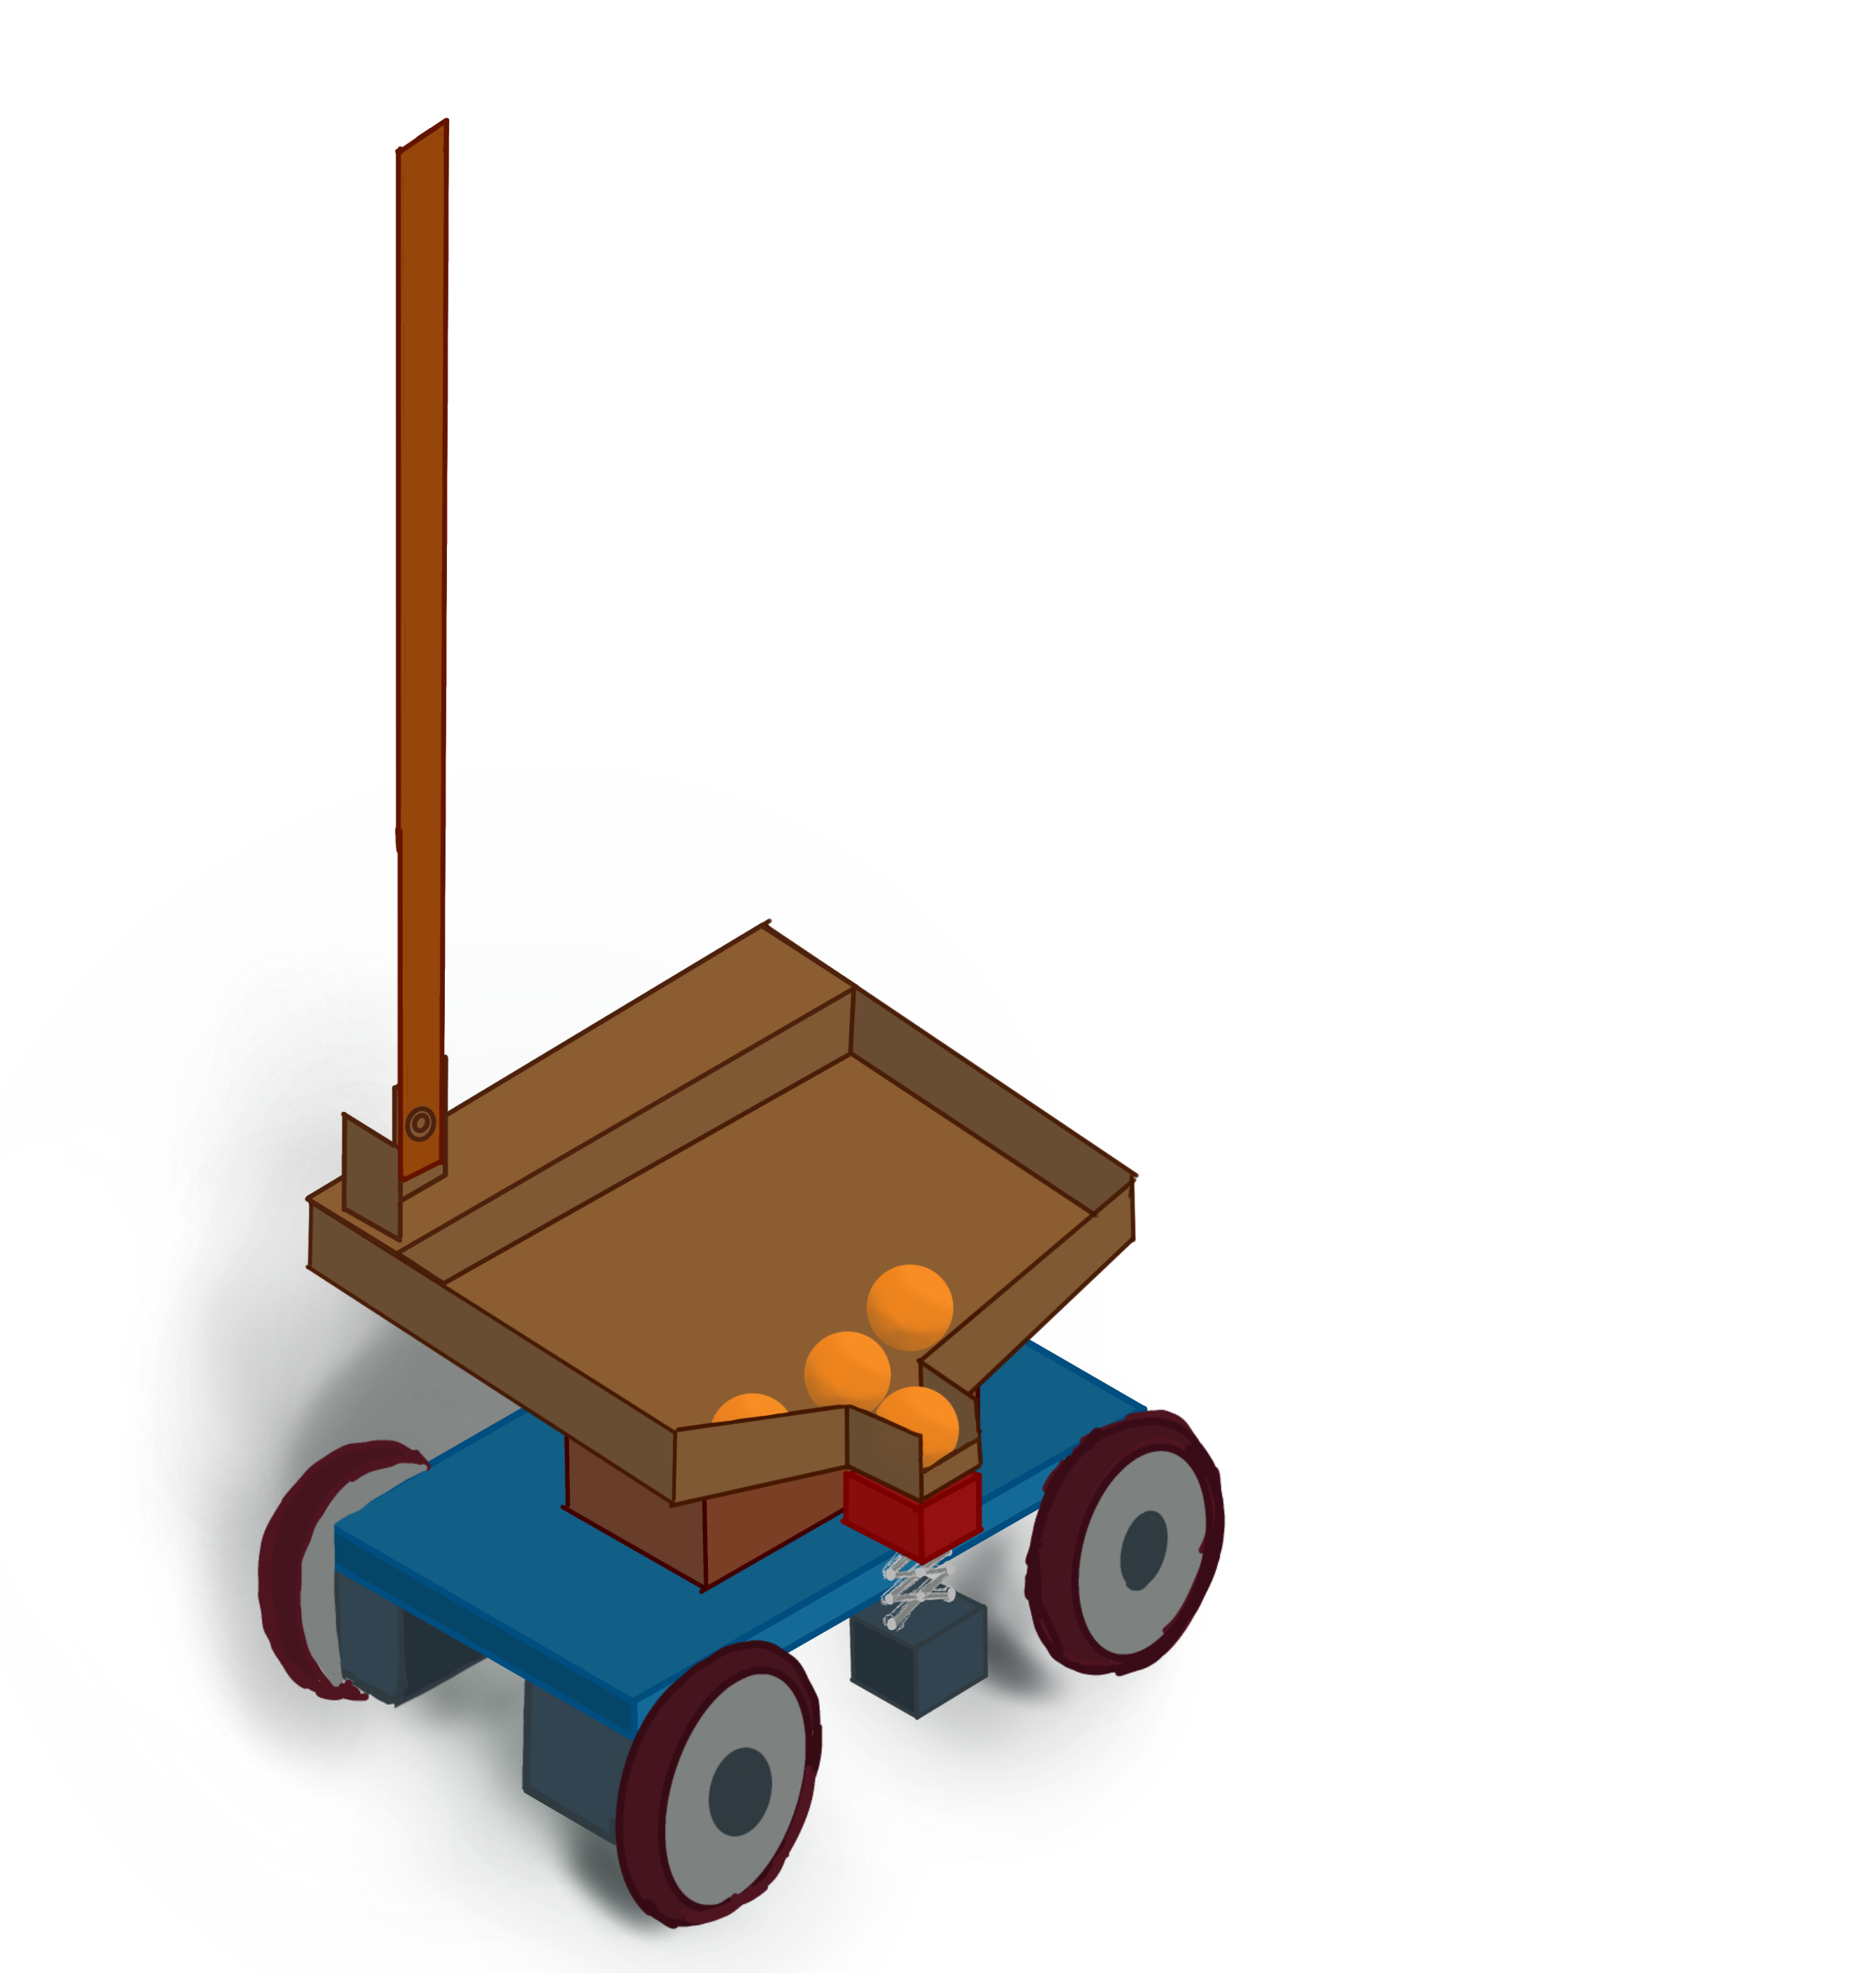
\includegraphics[width=3in]{海上形态1}
                    \caption{海上机器人初始状态}
                \end{minipage}
                \begin{minipage}[t]{0.48\textwidth}
                    \centering
                    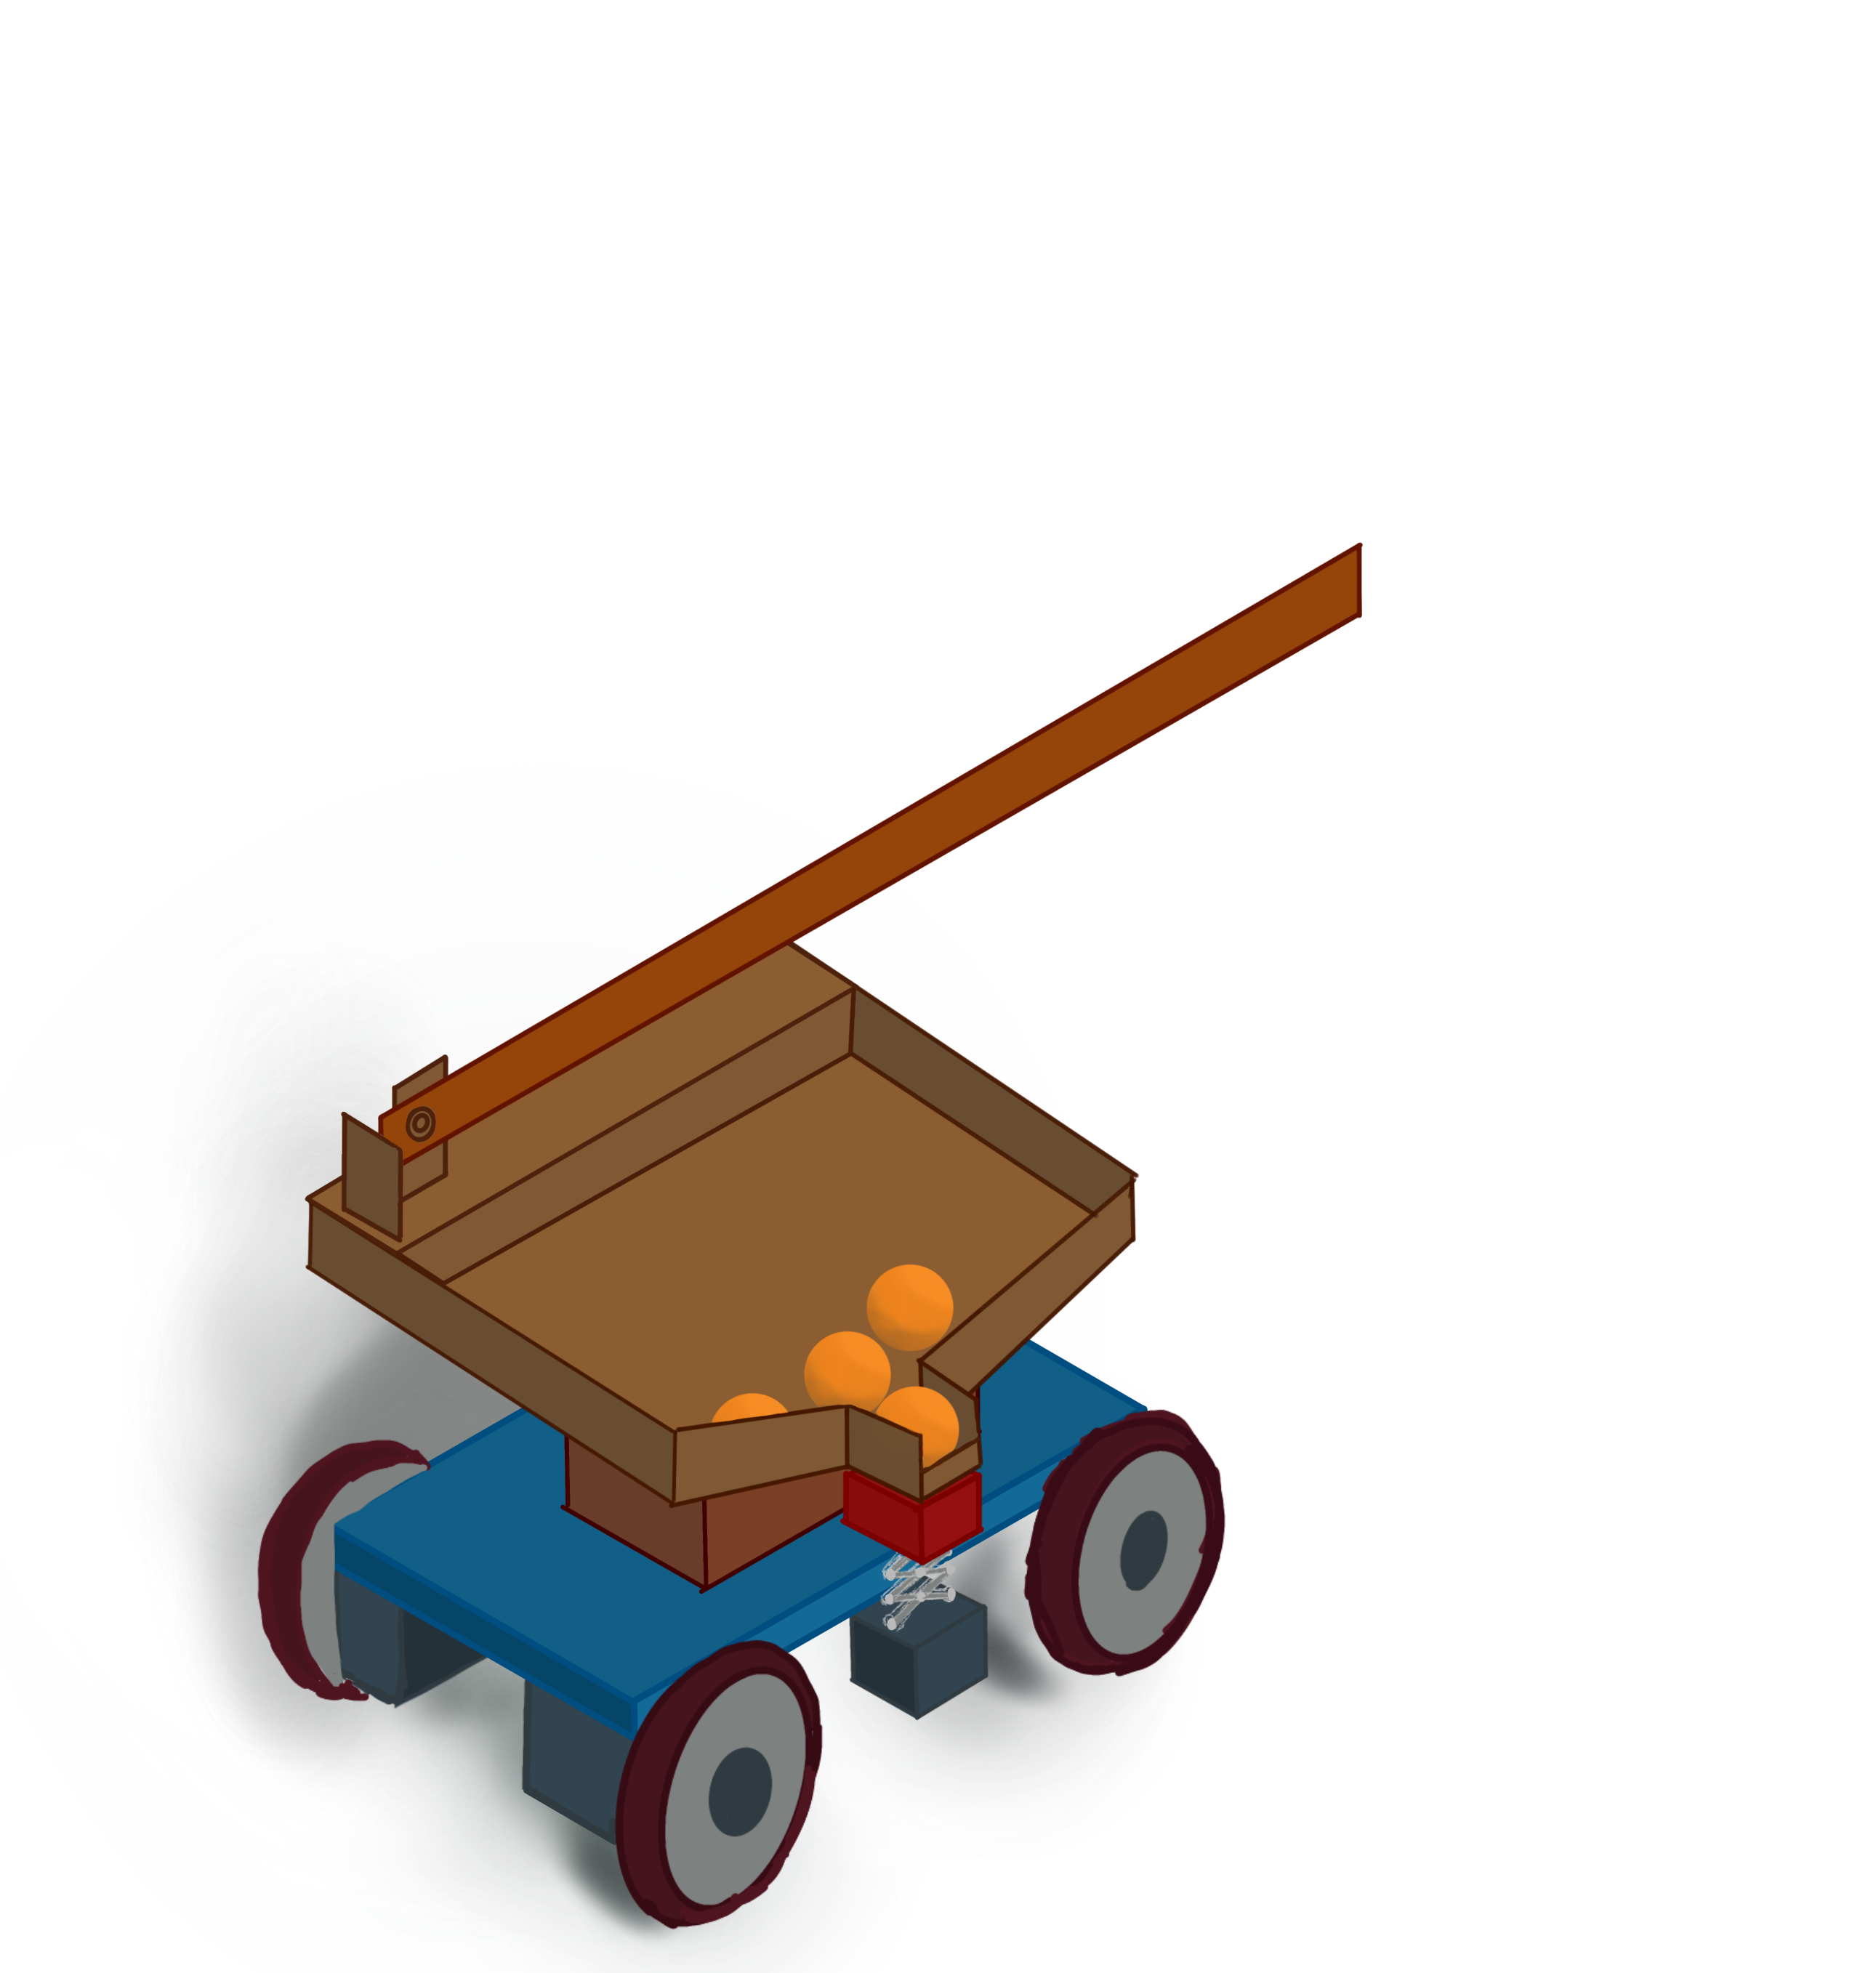
\includegraphics[width=3in]{海上形态2}
                    \caption{海上机器人干扰状态}
                \end{minipage}
            \end{figure}
            
        海上机器人由底盘、货物投放装置与干扰装置三部分组成。
        \par
        底盘部分,采用四轮结构,在前轮上安装一对电机与减速结构作为动力来源,机器人的转向则是控制电机转速不同进行差速转向,另外机器人的底盘上再搭载四路红外光电循迹传感器,以支持循迹功能——整个底盘结构,用于给上层结构提供支撑,稳定机身,提供前进、后退、转向功能,在无人控制的条件下能够循迹到达指定地点。
        \par
        货物投放装置由货物装载盒与升降机构成。货物装载盒是一个带有边缘围栏防止乒乓球掉出,内部向侧面中部一处倾斜的盒子,用于装载足够数量的货物,而整个装载盒的最低处与升降机结构结合,高度约为180mm,稍低于贸易区外边缘,构成货物投放装置。升降机结构则是嵌入于装载盒最低位置稍大于单个乒乓球的方块,方块上表面向外倾斜,收在装载盒围栏内部,方块底部利用连杆与舵机相连,可以在竖直方向上进行有限度的升降。
        升降装置工作时,分为三步:一、初始状态因为方块位于装载盒最底部,乒乓球自然滚落,只要装载盒不为空,方块上均会有且仅有一个乒乓球,且因为围栏的阻挡,乒乓球在机器人静止与行进时乒乓球不会掉出;二、当车辆行进至合适位置停下后,升降机结构可以开始工作,当方块上升超过装载盒围栏时,乒乓球顺着方块表面向外部的贸易区滑落,实现每次一个球的精准投放;三、收回方块回到原位置,等待新的乒乓球就位。升降装置的设计综合考虑了投放的精准程度与投放效率,最终通过消耗一个舵机的开销设计了该投放装置方案。
        \par
        而干扰装置则位于装载最高处的另一侧边缘,由一根可以绕固定点转动的长木条与一块限制转动方向的挡板构成,比赛开始前,将长木条竖直放置以满足机器人面积要求,当机器人开始行进,木条受到扰动倒下,成为可以扫落宝物的干扰结构。木条本身不存在动力结构,相对机器人固定,功能依靠跟随机器人移动实现。

        \subsection{陆上机器人}
        \begin{figure}[H]
            \centering
            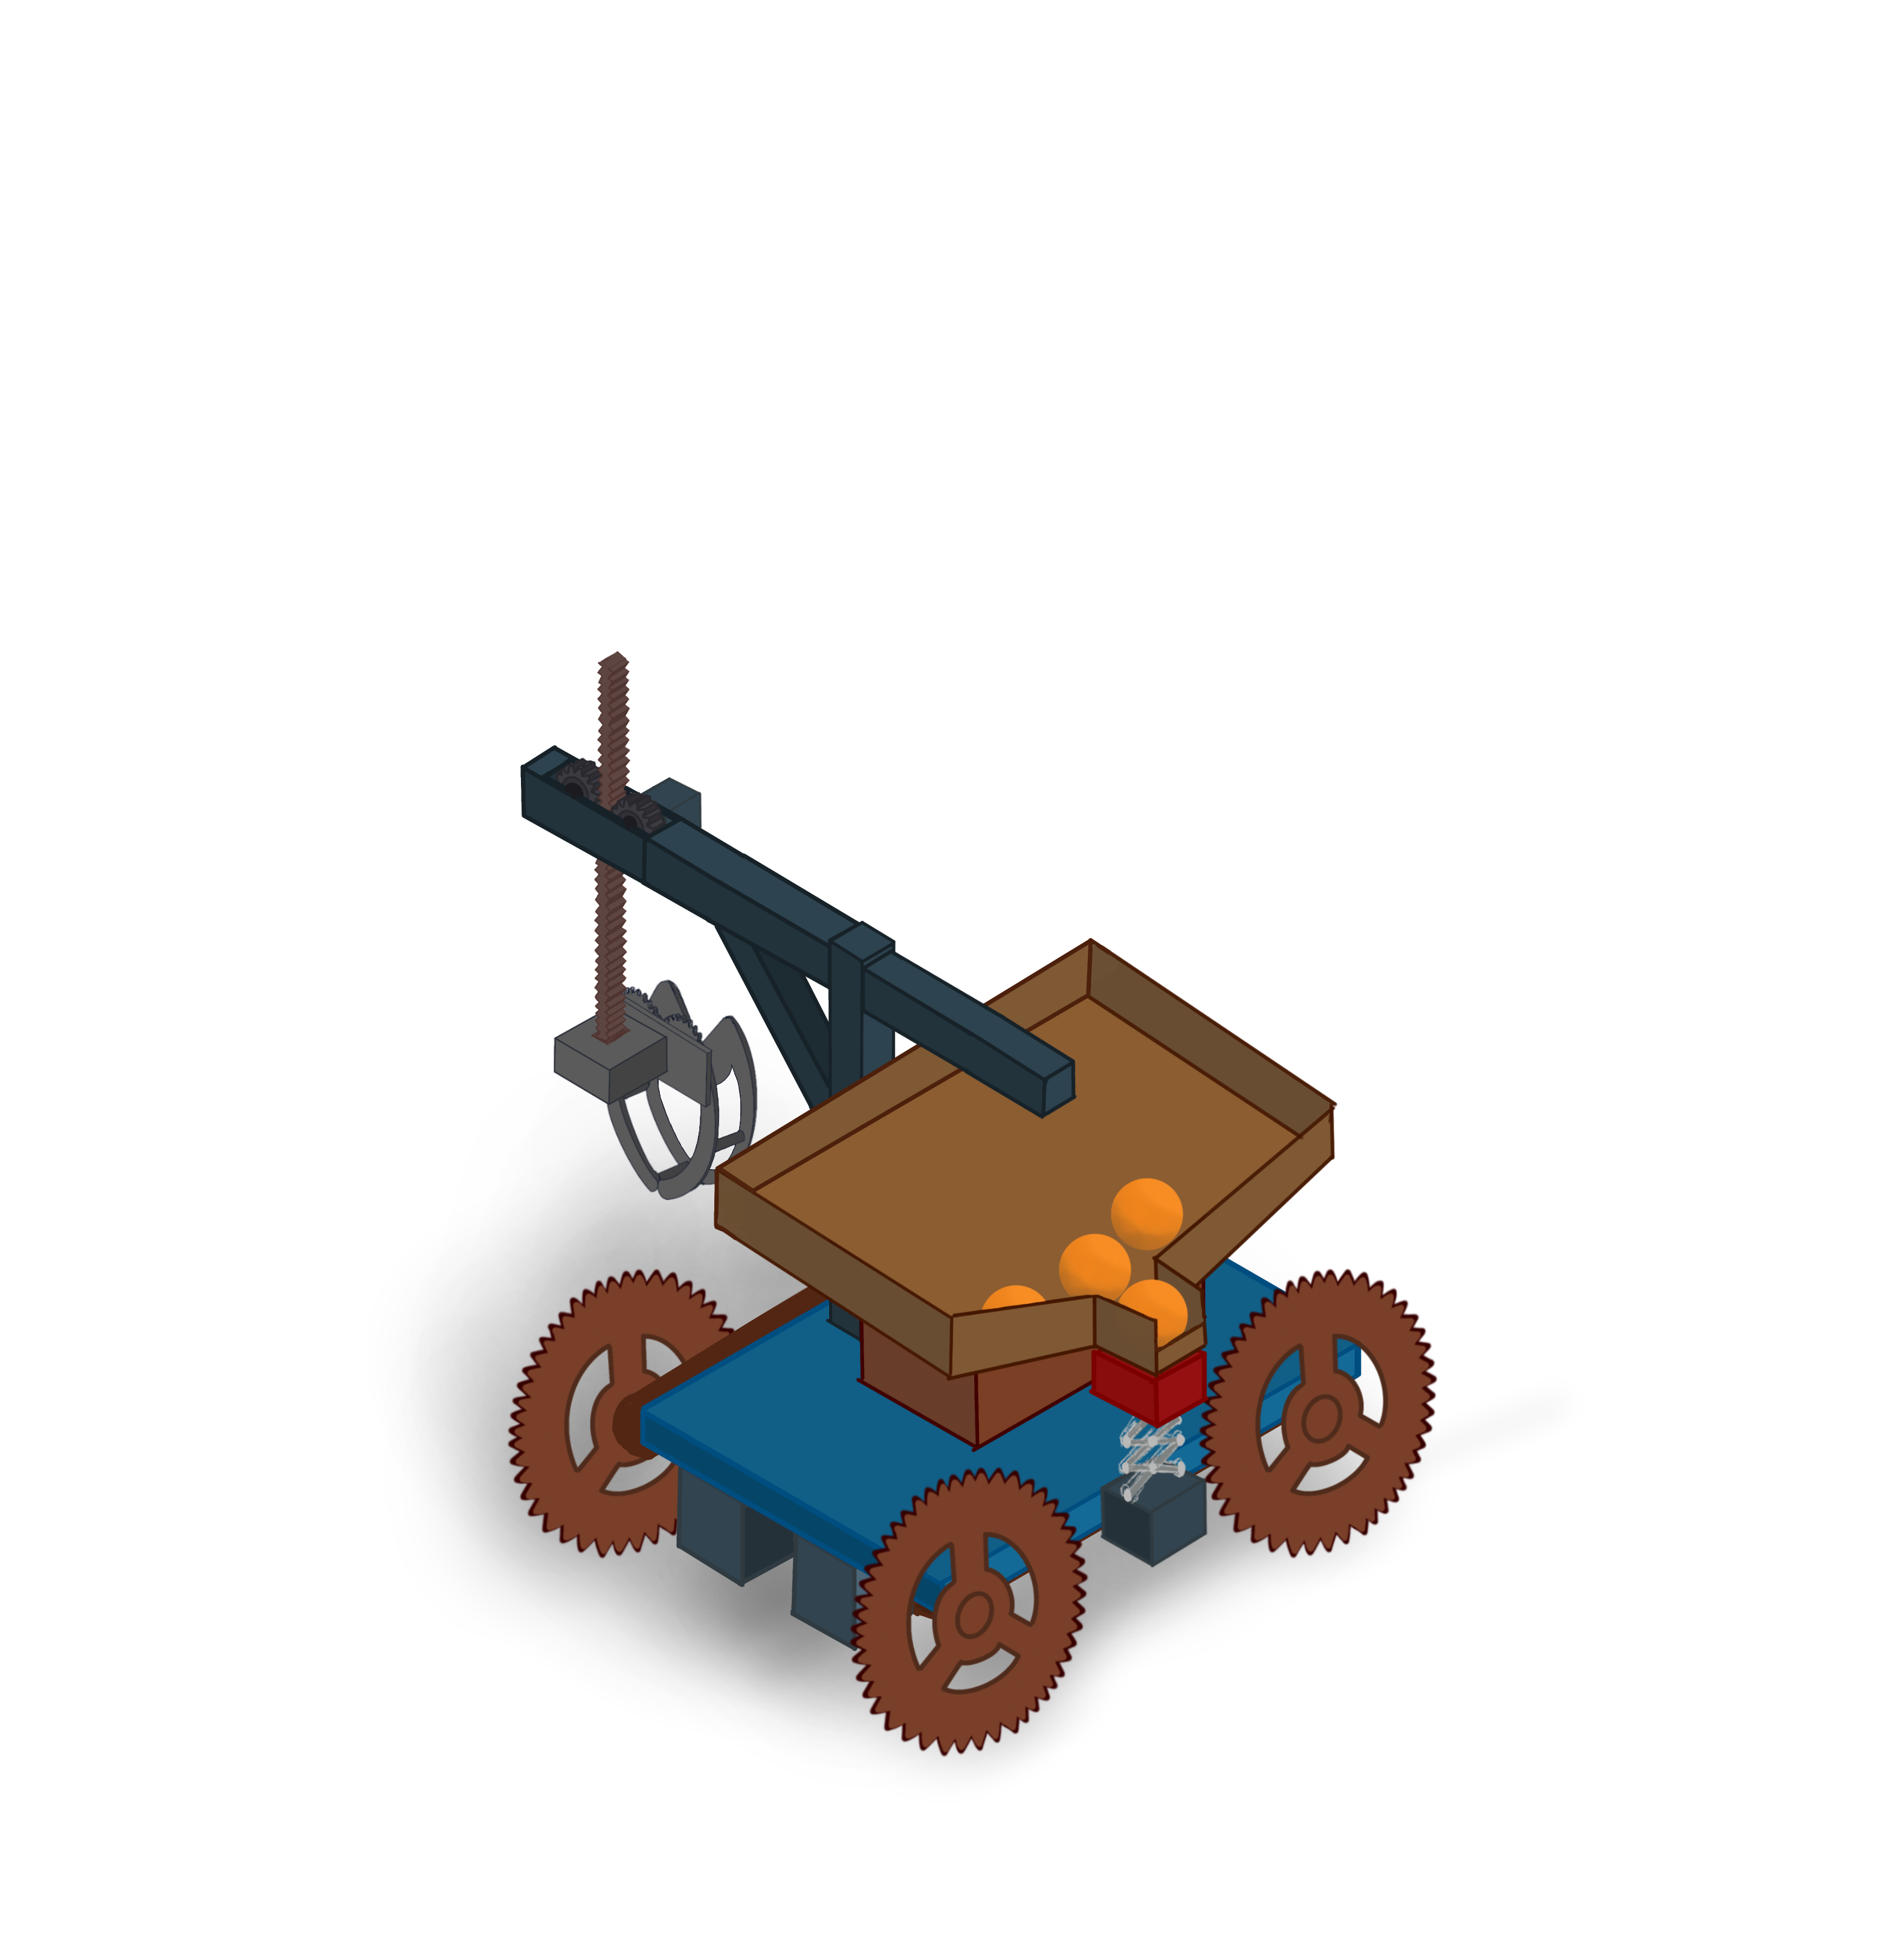
\includegraphics[width = 4in]{陆地形态}
            \caption{陆上机器人}
        \end{figure}
        陆上机器人由底盘、货物投放装置与塔吊结构三部分组成。
        \par
        底盘部分,由于存在攀爬40mm与30mm台阶的需求,除去基本的前进、后退与转向功能外,结构上的设计需要考虑攀登台阶的可靠性与效率。类似于海上机器人底盘,陆上机器人仍采用四轮驱动,差速转向,轮子为由木板加工而成的齿轮状,在行进到台阶时,轮齿可以于台阶直角突起上借力爬坡;一对电机与减速结构被安装于前轮上,四轮的轮轴上均带有齿轮结构,底盘两侧的前后轮的轮轴通过链条相连,能够将前轮的动力传递到后轮,使得爬坡时后轮仍能够提供动力帮助机器人顺利爬坡。另外,由于吊机结构可能导致重心过高与不稳定的问题,底盘上可根据实际情形在不影响爬坡的前提下添加配重稳定机身。
        \par
        货物投放装置:整体结构与海上机器人的货物投放装置一致,且由于陆上需要投放的货物量少,装载盒面积可以压缩,底盘上腾出的空间用于安装塔吊装置,考虑比赛地图上交易区与放置宝物的立柱间距离约为450mm,利用前后方向进行货物放置转向较为困难,货物投放与吊机可分别朝向机器人的左右方向,使得向交易区内投放至少一个货物后能够通过前进与后退的同时转向调整姿态,快速进入抓取宝物的状态。
        \par
        塔吊结构:塔吊结构由两根互相垂直的长杆、支撑结构、升降结构与抓取结构组成。
        两根垂直长杆于交叉点处固定连接,且于该点处引出一斜拉绳固定于底盘上,用于防止塔吊结构向外倾倒,另用一根支撑杆令两垂直杆间构成三角结构,防止发生转动,使横杆保持稳定。
        升降结构主要由一根只能在竖直方向上运动的杆与齿条构成,由舵机与齿轮驱动齿条控制杆上下升降。
        \par
        抓取结构由固定在升降机结构上的两个相互啮合的齿轮与舵机构成,两个互相啮合的齿轮可以实现开合效果,齿轮带动抓机械爪,机械爪内部加有高阻尼材料,令抓取稳定。

    \section{关键部分零件图}

        \subsection{升降装置状态分解}
        \begin{figure}[H]
            \centering
            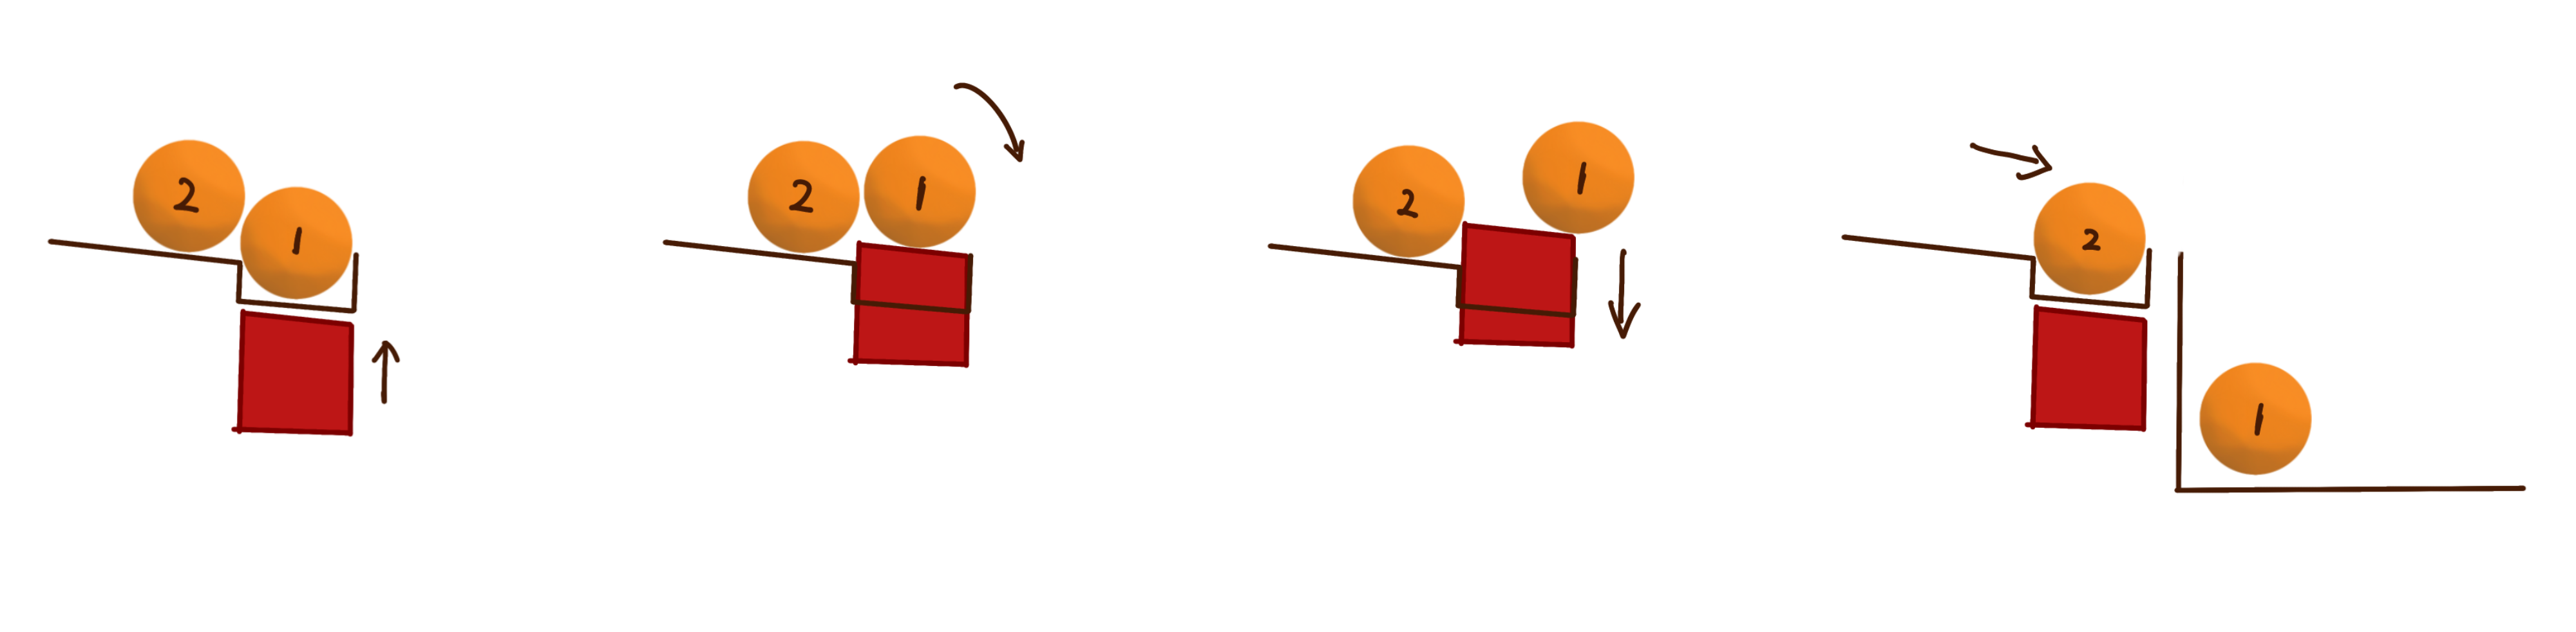
\includegraphics[width = 6in]{分解}
            \caption{陆上机器人}
        \end{figure}  
        \subsection{塔吊结构}
        \begin{figure}[H]
            \centering
                \begin{minipage}[t]{0.48\textwidth}
                    \centering
                    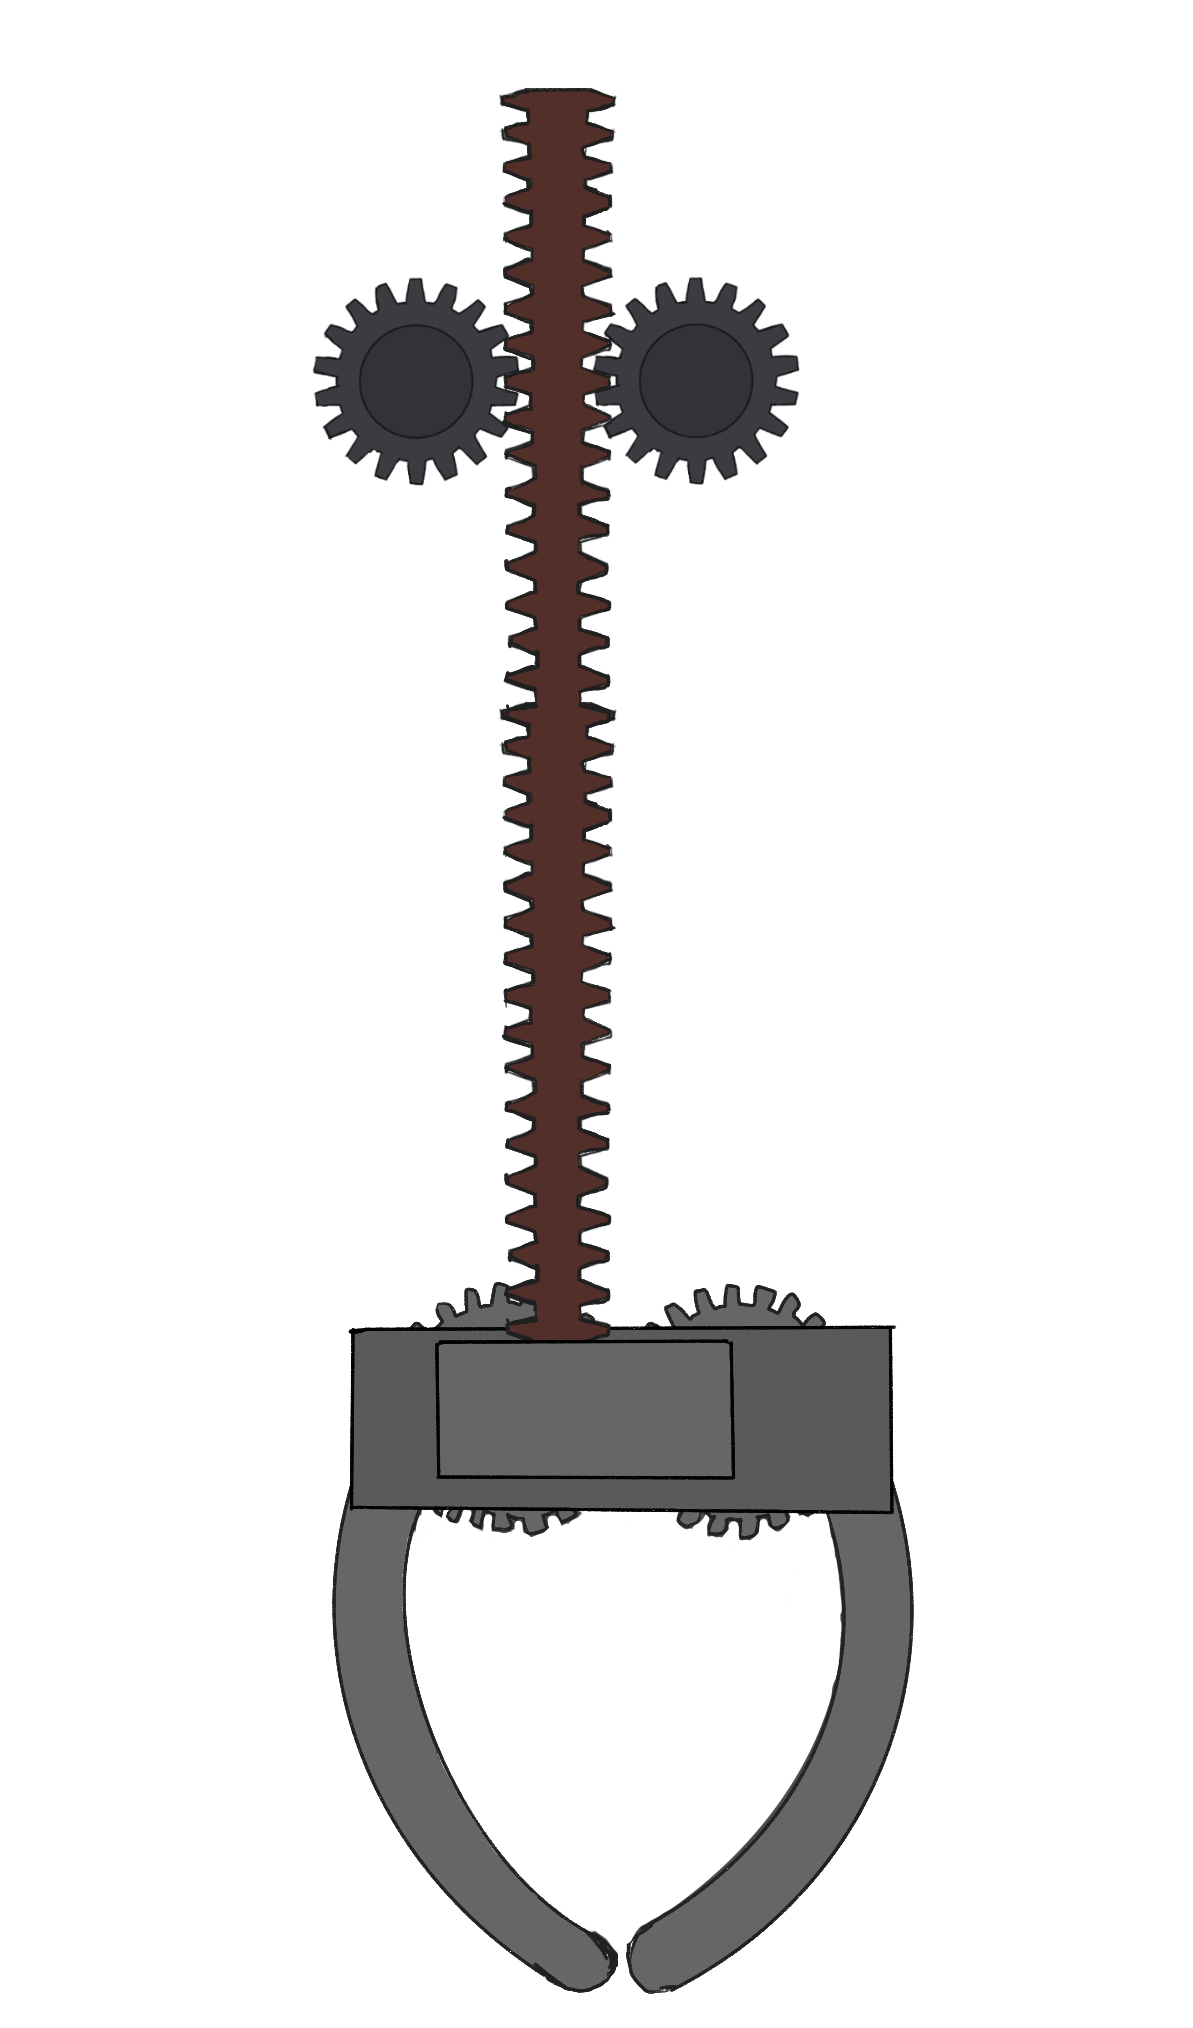
\includegraphics[width=1.5in]{claw1}
                    \caption{海上机器人初始状态}
                \end{minipage}
                \begin{minipage}[t]{0.48\textwidth}
                    \centering
                    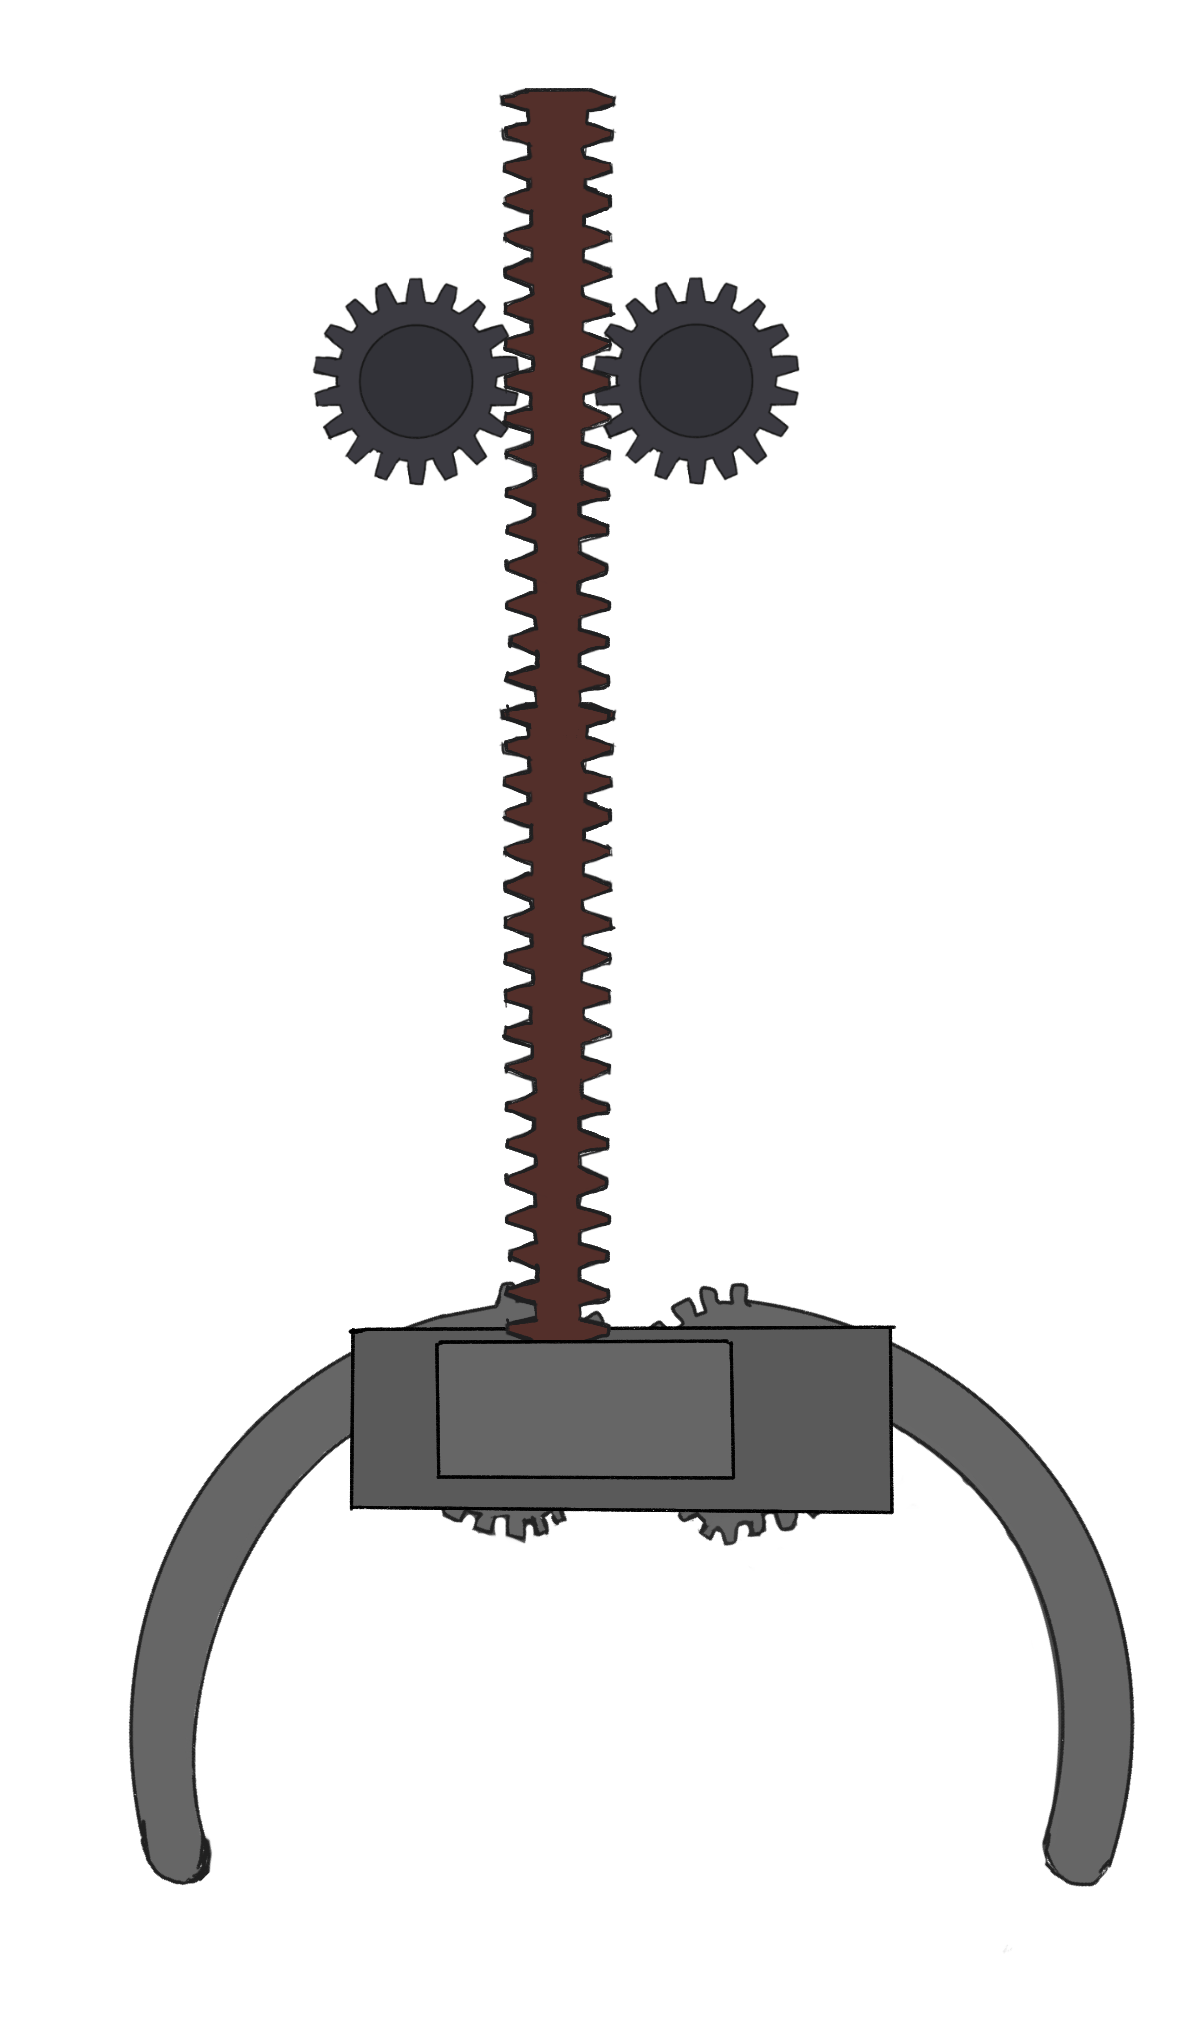
\includegraphics[width=1.5in]{claw2}
                    \caption{海上机器人干扰状态}
                \end{minipage}
            \end{figure}
    \section{通信控制}

    海上机器人:
    \par
    海上机器人电路主要用于驱动控制行进的两个电机、一个控制升降机的舵机以及无线通信模块用于使用遥控器实现对小车的控制。由于软件封装等原因,无线通信模块在下文不表。
    \par
    使用stm32单片机上的四个数字输出为两个电机的信号输入。两个电机通过L298N和STM32实现对电机转速转向的控制
    \begin{table}[H]
        \centering
        \begin{tabular}{|c|c|c|}
        \hline
        转向 & In1 & In2 \\ \hline
        正传 & 高   & 低   \\ \hline
        反转 & 低   & 高   \\ \hline
        停止 & 低   & 低   \\ \hline
        停止 & 高   & 高   \\ \hline
        \end{tabular}
    \end{table}
    舵机的控制则直接将舵机与STM32共地,并将信号端口与其相连即可
    \par
    陆地机器人:
    \par
    陆地机器人与海上机器人相似,唯一区别则是陆地机器人需要多控制塔吊结构中的两个舵机,以实现抓取的功能

    \section{耗材分析}

    海上机器人共消耗2个电机1个舵机,陆上机器人共消耗2个电机3个舵机,满足电机数量小与等于8个的限制。
    陆上机器人前后轮传动的链条选择通过100元的经费购买。
    其余耗材所给出的清单均能满足需求。

    \section{思考与感想}

        \subsection{杨子晗}
        我在本次机器人设计的过程中,体会到了合作讨论的重要性,一次次的讨论中,新的方案不断被提出,又不断被否决替代,最终得到的方案混合了所有人的思考,这个一个令人兴奋与愉快的过程。另外作为一名计算机科学与技术专业的学生,大作业面向的领域和工作与我平时所学的完全不同,很多地方都需要从零学起,整个设计报告完成的过程也是我不断学习提升的过程,在这个过程中我学到了很多新的知识与解决问题的思考方式,受益匪浅。
        \subsection{周灿松}
        \subsection{姚桂涛}
        这次机器人大作业让我收获颇多。首先是对于比赛规则的理解,由于比赛规则书是英文的,所以导致开始的理解上会有一些困难。但是在边理解边和小组成员讨论的过程中,很快就对比赛规则有了很好的理解。其次,在讨论比赛的战术策略,机器人设计时,小组成员进行头脑风暴,涌现了许多有趣新颖的想法。在熟悉了比赛规则以及有了初步的想法之后,我们便进行了明确的分工。有了明确的分工后,我们的进度大大加快。但是在设计初期,我们打算用专业绘图软件如solidworks进行3d图的绘制,但是在考虑到要学习掌握一个全新的软件要花费不短的时间后,便放弃了这个想法。而我有一定的绘画基础,于是我们决定由我来手绘参考图。绘图是一个从无到有的工作,由于没有实物参考,非常的困难。于是我便加强了和组员的讨论,边绘制草图边讨论细节,最终才画出了参考图。在这整个过程中,我加深了对机器人各种功能的理解,提升了自己的绘图能力。
        \subsection{邓智城}
        机器人设计的大作业是有趣而富有挑战性的。在策略规划过程中,大家一起进行头脑风暴,在规则约束之内思考出了很多“超脱规则”的想法。当然,这些想法并不只是新奇,更重要的是非常有用,可以获取更高的分数。小组最初打算全员学习SolidWorks用以绘制机器人图,但发现学习成本较高。同时,每人都负责绘图,就失去了team的意义。一个小组应该各司其职,发挥优势,各取所长,才能更好的完成任务。于是我们放弃了SolidWorks。在商谈完策略后,分工就开始明确了。我个人能力相对较弱,队伍里负责绘图和PPT的同学也十分优秀,于是我负责了汇总报告。集总大家的idea,将小组的成果尽量全面呈现出来。在本次合作中,和大家一起努力的感觉很不错。大家各司其职,很好地完成了大作业。
    
    \section{分工情况}

\end{document}